\chapter{一元函数微分学}
\section{导数和微分}
\centering{\textbf{练习题}}
\begin{enumerate}
    \item 用定义求$f'(0)$, 这里$f(x)=\begin{cases}
    x^2sin\frac{1}{x},&x\ne 0\\
    0,&x=0
    \end{cases}$
    \item 设$f'(x_0)$存在.求证:对数导数也存在并等于$f'(x_0)$, 即\\
    $$\lim\limits_{h\rightarrow 0}\frac{f(x_0+h)-f(x_0-h)}{2h}=f'(x_0)$$.
    \item 设$f(x)$在点$x_0$处可导,$\alpha_n,\beta_n$为趋于零的正数序列, 求证: 
    $$\lim\limits_{n\rightarrow \infty}\frac{f(x_0+\alpha_n-f(x_0+\beta_n))}{\alpha_n-\beta_n}
    = f'(x_0)$$
    \item 设$P(x)$是最高次项系数为1的多项式, $M$是它的最大实数.求证:$P'(M)\ge 0$.
    \item 给定曲线$y=x^2+5x+4$.
    \begin{enumerate}
    	\item 求曲线在点$(0,4)$处的切线.
    	\item 确定$b$使得直线$y=3x+b$为曲线的切线;
    	\item 求过点$(0,3)$的曲线的切线.
    \end{enumerate}
	\item 确定常数$a,b$使得函数$f(x)=\begin{cases}
	ax+b,&x>1\\
	x^2,&x\le 1
	\end{cases}$
	有连续导数.
	\item 设曲线由隐式方程$\sqrt[3]{x^2}+\sqrt[3]{y^2}=\sqrt[3]{a^2}(a>0)$给出.
	\begin{enumerate}
		\item 求证: 曲线的切线被坐标轴所截的长度为一常数;
		\item 写出曲线的参数式, 利用参数式求导给出上一小题的另一证法.
	\end{enumerate}
		\item 已知曳物线的参数方程为$$
		x=a[\mathrm{ln}(\mathrm{tan}\frac{t}{2})+\mathrm{cos}t],\quad y=a\mathrm{sin}t\quad
		(a>0,0<t<\pi).$$
		求证:在曳物线的任意切线上, 自切点至该切线与$x$轴交点之间的切线段为一定长.
		\item 试确定$\lambda$,使得曲线$\frac{x^2}{a^2}+\frac{y^2}{b^2}$与$xy=\lambda$相切, 并求出切线方程.
		\item 试确定$m$, 使直线$y=mx$为曲线$y=lnx$的切线.
		\item 设$y=\frac{\mathrm{arcsin}x}{\sqrt{1-x^2}}$.
		$(1)\text{求证}: (1-x^2)y'-xy=1;\qquad \quad(2)\text{求}y^{(n)}(0)$.
		\item 求$f(x)=\frac{x}{1-x^2}$的$n$阶导数.
		\item 设$y=x^(n-1)\mathrm{ln}x$.求证:$y^{(n)}=\frac{(n-1)!}{x}$.
		\item 求证:双曲线$r^2=a^2\text{cos}2\theta$的向径与切线的夹角等于极角的两倍加$\frac{\pi}{2}$
		\item 设曲线既可用参数式$x=x(t),y=y(t)$表示, 又可用极坐标$r=r(\theta)$表示.求证:$\frac{1}{2}r^2\mathrm{d}\theta=\frac{1}{2}(x\mathrm{d}y-y\mathrm{d}x)$.
		
	\end{enumerate}
\section{微分中值定理}
\centering{\textbf{练习题}}
\begin{enumerate}
	\item 设$f(x)$在$[a,b]$上连续, 在$(a,b)$内除仅有的一个点都可导.求证: $\exists c_1,c_2\in(a,b)$及$\theta \in (0,1)$, 使得
	$$f(b)-f(a)=(b-a)[\theta f'(c_1)+(1-\theta)f'(c_2)]
	$$
	\item 设函数$f(x)$在$[a,b]$上连续, 在$(a,b)$内可导, 且$$
	f(a)\cdot f(b) > 0,\ f(a)\cdot f(\frac{a+b}{2})<0.$$
	求证: 对$\forall k\in R, \exists \xi\in (a,b)$, 使得$f'(\xi)=kf(\xi)$.
	\item 设$f(x)$在$[a,b]$上连续, 在$(a,b)$内可导, 但非线性函数. 求证: 
	$\exists \xi,\eta\in(0,3), $使得$f'(\xi)=0$.
	\item 设$f(x)$在$[a,b]$上连续, 在$(a,b)$内可导, 但非线性函数.求证: $\exists \xi,\eta\in (a,b)$,使得$$
	f'(\xi)<\frac{f(b)-f(a)}{b-a}<f'(\eta).$$
	\item 设$f(x)$在$(a,b)$内二阶可导,且$x_0\in (a,b)$, 使得$f''(x_0)\ne 0$.求证:
	\begin{enumerate}
		\item 如果$f'(x_0)=0$,则存在$x_1,x_2\in (a,b)$,使得${f(x_1)-f(x_2)}=0$;
		\item 如果$f'(x_0)\ne 0$, 则存在$x_1,x_2\in (a,b)$, 使得$\frac{f(x_1)-f(x_2)}{x_1-x_2}=f'(x_0)$.
	\end{enumerate}
	\item 设$f(x)$在$[0,1]$上可导, $f(0)=0, f(x)\ne 0(\forall x\in(0,1))$.求证: 如果$f(x)$在$(0,1)$上不恒等于零, 则存在$\xi \in (0,1)$, 使得$f(\xi)\cdot f'(\xi)>0$.
	\item 设$f(x)$在$[0,1]$上可导,$f(0)=0,f(x)\ne 0(\forall x\in (0,1))$.求证:
	存在$\xi\in(a,b)$, 使得$f'(\xi)+f(\xi)=0$.
	\item 设$f(x)$在$[0,1]$上连续,在$(0,1)$内可导,$f(0)=0$.求证:如果$f(x)$在$(0,1)$上不恒等于零,则存在$\xi \in (0,1)$, 使得$f(\xi)\cdot f(\xi)>0$.
	\item 设函数$f(x)$在$[a,b]$上可导, 且$f'(a)=f'(b)$.求证: $\exists c\in (a,b), $使得$f(c)-f(a)=(c-a)f'(c)$ \\
	注:\quad 本题与本节例12比较,就是把条件$f'(a)=f'(b)=0$中的“=0”去掉了.
	\item 设$f(x)$在(0,1]上可导, 且存在有限极限$\lim\limits_{h\rightarrow 0+}\sqrt{x}f'(x)$.求证:$f(x)$在(0,1]上一致连续.
\end{enumerate}

\section{函数的升降、极值、最值问题}
\centering\textbf{练习题}
\begin{enumerate}
	\item 求证: 
	\begin{enumerate}
		\item 当$x\ge 0$时, $f(x)=\frac{x}{1+x}$单调增加;
		\item $\frac{|a+b|}{1+|a+b|}\le \frac{|a|}{1+|a|}+\frac{|b|}{1+|b|}$.
	\end{enumerate}
		\item 设$f(x)$在$[0,a]$上二次可导, 且$f(0)=0, f''(x)<0$.求证: $\frac{f(x)}{x}$在$(0,a]$上单调下降.
		\item 求证: 对任何$n(n>0)$次多项式$P(x),\exists x_0>0$,使得$P(x)$在$(-\infty,-x_0)$和在$(x_0,+\infty)$上都是严格单调的.
		\item 设$f(x)$在$[a,b]$上连续, 且在$(a,b)$内只有一个极大值点和一个极小值点. 求证: 极大值必大于极小值.
		\item 设$a,b>0,k\in R$.求证: 函数$f(x)=a^2e^{kx}+b^2e^{-kx}$存在与$k$无关的极小值.
		\item 
		\begin{enumerate}
			\item 设$f(x), g(x)$在$(a,b)$内可导, 且$f(x)\ne g(x),g(x)\ne 0$.求证: $\frac{f(x)}{g(x)}$在$(a,b)$内无极值的充分必要条件是$\frac{f(x)+g(x)}{f(x)-g(x)}$在$(a,b)$内无极值.
			\item 设$b>a>0$, 求证: $f(x)=\frac{(x-a)(x+b)}{(x-b)(x+a)}$无极值.
		\end{enumerate}
\begin{minipage}[b]{0.55\linewidth}
	\item 设函数$f(x)$在$(-\infty,+\infty)$内连续, 其导函数的图形如图2.4所示, 则$f(x)$有(\ ).\\
		\text{\qquad} (A)一个极小值和两个极大值;\\
		\text{\qquad} (B)两个极小值和一个极大值;\\
		\text{\qquad} (A)两个极小值和两个极大值;\\
		\text{\qquad} (A)三个极小值和一个极大值;
\end{minipage}
\hfill
\begin{minipage}[b]{0.65\linewidth}
	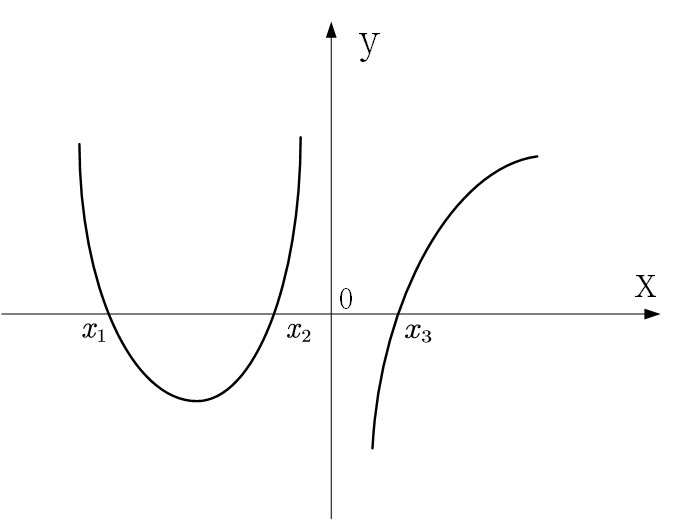
\includegraphics[height=5\baselineskip]{picture2_4.jpg}\\
	\text{\qquad \quad} 图2.4
\end{minipage}
\item 
\begin{enumerate}
	\item 求证:序列$\{\frac{\mathrm{ln}n}{n}\}_{n=3}^{\infty}$为一递减序列;
	\item 求序列$\{\sqrt[n]{n}\}$的最大项.
\end{enumerate}
	\item 假设$f(x)=1+x+\frac{x^2}{2!}+\cdots+\frac{x^{2n}}{(2n)!}$.求证:$f(x)$在实轴上有真正得最小值.
	\item 设$f(x)\in C[a,b]$,在区间$[a,b]$上只有一个极值点.求证: 如果该点是极大值点必为最大值点; 如果该点是极小值点必为最小值点.
	\item 求出满足不等式$\frac{B}{\sqrt{x}}\le \mathrm{ln}x \le A\sqrt{x}\ (\forall\ x>0)$的最小正数$A$及最大负数$B$.
	\item 给定曲线$y=\frac{1}{\sqrt{x}}(x>0)$.
	\begin{enumerate}
		\item 求过点$(x_0,\frac{1}{\sqrt{x_0}})$的切线.
		\item 在曲线上求一个点, 使曲线在该点处的切线在$x$轴与$y$轴上截距和最小.
	\end{enumerate}
	\item 设正数$x,y$之和为一常数$2a(a>0)$, 且指数$x^y$当$x=a$时, 达到最大值. 求证: $a=e$.
	\item 给定曲线$y=\frac{1}{x^2}$.
	\begin{enumerate}
		\item 求曲线上横坐标为$x_0$的点处的切线方程;
		\item 在曲线上求一个点, 使曲线在该点处的切线被坐标轴所截的长度最短.
	\end{enumerate}
	\item 做一个无盖的圆柱形茶缸, 若体积$V$一定, 问底半径$R$与高$H$成何比例时, 使总面积最小(即用料最省) ?
	\item 有一半径为$a$的半球面形的杯子, 杯内放一长度为$l(l>2a)$的均匀细棒, 求棒的平衡位置(即求棒重心的最低位置).
	\item 把一圆形铁片剪下中心角为$\alpha$的一块扇形部分, 并将其围成一圆锥. 已知圆形铁片的半径为$R$, 问$\alpha$多大时, 圆锥的容积最大?
\end{enumerate}

\section{函数的凹凸性、拐点及函数作图}
\centering{\textbf{练习题}}
\begin{enumerate}
	\item 设$a>0,b>0$.求证: $f(x)=\sqrt{a+bx^2}$为凹函数.
	\item 求证: 不存在三次或三次以上的奇次多项式为凹函数.
	\item 设$f(x)$在$(a,b)$上取正值, 且为凸函数.求证: $\frac{1}{f(x)}$是在$(a,b)$上的凹函数.
	\item 设$f(x)$在$[a,+\infty)$上二次可微,$f''(x)\ge 0$.求证:
	\begin{enumerate}
	\item $\frac{f(x)-f(x-h)}{h}\in f'(x)\in \frac{f(x+h)-f(x)}{h}(0<h<x)$;
	\item 若$\lim\limits_{x\rightarrow +\infty}\frac{f(x)}{x}=1$, 则$\lim\limits_{n\rightarrow +\infty}f'(x)=1$.
	\end{enumerate}
	\item 作出下列函数的图形:
	\begin{table}[H]
		\begin{tabular}{ll}
			\qquad	(1)\ $y=x^3-x^2-x+1$;\qquad \qquad& (2)\ $y=x\cdot e^{-x^2}$;\\
			\qquad (3)\ $y=x+\frac{1}{x}$; \qquad \qquad &(4)\ $y=x\cdot \mathrm{ln}x$.
		\end{tabular}
	\end{table}

\end{enumerate}

\section{洛必达法则与泰勒公式}

\section{一元函数微分学的总合应用}